\documentclass{article}

\usepackage{fancyhdr}
\usepackage{extramarks}
\usepackage{amsmath}
\usepackage{amsthm}
\usepackage{amsfonts}
\usepackage{tikz}
\usepackage[plain]{algorithm}
\usepackage{algpseudocode}
\usepackage{pgfplots}

\usetikzlibrary{automata,positioning}

%
% Basic Document Settings
%

\topmargin=-0.45in
\evensidemargin=0in
\oddsidemargin=0in
\textwidth=6.5in
\textheight=9.0in
\headsep=0.25in

\linespread{1.1}

\pagestyle{fancy}
\lhead{\hmwkAuthorName}
\chead{\hmwkClass:\ \hmwkTitle}
\rhead{\firstxmark}
\lfoot{\lastxmark}
\cfoot{\thepage}

\renewcommand\headrulewidth{0.4pt}
\renewcommand\footrulewidth{0.4pt}

\setlength\parindent{0pt}
\setlength{\parskip}{5pt}

%
% Create Problem Sections
%

\newcommand{\enterProblemHeader}[1]{
    \nobreak\extramarks{}{Problem \arabic{#1} continued on next page\ldots}\nobreak{}
    \nobreak\extramarks{Problem \arabic{#1} (continued)}{Problem \arabic{#1} continued on next page\ldots}\nobreak{}
}

\newcommand{\exitProblemHeader}[1]{
    \nobreak\extramarks{Problem \arabic{#1} (continued)}{Problem \arabic{#1} continued on next page\ldots}\nobreak{}
    \stepcounter{#1}
    \nobreak\extramarks{Problem \arabic{#1}}{}\nobreak{}
}

\setcounter{secnumdepth}{0}
\newcounter{partCounter}
\newcounter{homeworkProblemCounter}
\setcounter{homeworkProblemCounter}{1}
\nobreak\extramarks{Problem \arabic{homeworkProblemCounter}}{}\nobreak{}

%
% Homework Problem Environment
%
% This environment takes an optional argument. When given, it will adjust the
% problem counter. This is useful for when the problems given for your
% assignment aren't sequential. See the last 3 problems of this template for an
% example.
%
\newenvironment{homeworkProblem}[1][-1]{
    \ifnum#1>0
        \setcounter{homeworkProblemCounter}{#1}
    \fi
    \section{Problem \arabic{homeworkProblemCounter}}
    \setcounter{partCounter}{1}
    \enterProblemHeader{homeworkProblemCounter}
}{
    \exitProblemHeader{homeworkProblemCounter}
}

%
% Homework Details
%   - Title
%   - Due date
%   - Class
%   - Section/Time
%   - Instructor
%   - Author
%

\newcommand{\hmwkTitle}{Homework\ \#1}
\newcommand{\hmwkDueDate}{October 16, 2023}
\newcommand{\hmwkClass}{ECE 271A}
\newcommand{\hmwkClassInstructor}{Professor Vasconcelos}
\newcommand{\hmwkAuthorName}{\textbf{Ray Tsai}}
\newcommand{\hmwkPID}{A16848188}

%
% Title Page
%

\title{
  \vspace{2in}
  \textmd{\textbf{\hmwkClass:\ \hmwkTitle}}\\
  \normalsize\vspace{0.1in}\small{Due\ on\ \hmwkDueDate\ at 11:59pm}\\
  \vspace{0.1in}\large{\textit{\hmwkClassInstructor}} \\
  \vspace{3in}
}

\author{
  \hmwkAuthorName \\
  \vspace{0.1in}\small\hmwkPID
}
\date{}

\renewcommand{\part}[1]{\textbf{\large Part \Alph{partCounter}}\stepcounter{partCounter}\\}

%
% Various Helper Commands
%

% Useful for algorithms
\newcommand{\alg}[1]{\textsc{\bfseries \footnotesize #1}}

% For derivatives
\newcommand{\deriv}[1]{\frac{\mathrm{d}}{\mathrm{d}x} (#1)}

% For partial derivatives
\newcommand{\pderiv}[2]{\frac{\partial}{\partial #1} (#2)}

% Integral dx
\newcommand{\dx}{\mathrm{d}x}

% Probability commands: Expectation, Variance, Covariance, Bias
\newcommand{\Var}{\mathrm{Var}}
\newcommand{\Cov}{\mathrm{Cov}}
\newcommand{\Bias}{\mathrm{Bias}}
\newcommand*{\Z}{\mathbb{Z}}
\newcommand*{\Q}{\mathbb{Q}}
\newcommand*{\R}{\mathbb{R}}
\newcommand*{\C}{\mathbb{C}}
\newcommand*{\N}{\mathbb{N}}
\newcommand*{\prob}{\mathds{P}}
\newcommand*{\E}{\mathds{E}}

\begin{document}

\maketitle

\pagebreak

\begin{homeworkProblem}
  In this problem we will consider the traditional probability scenario of coin tossing. However, we
  will consider two variations. First, the coin is not fair. Denoting by $S$ the outcome of the coin toss we
  have
  \[
    P_S(heads) = \alpha, \alpha \in [0, 1].
  \]
  Second, you do not observe the coin directly but have to rely on a friend that reports the outcome of
  the toss. Unfortunately your friend is unreliable, he will sometimes report heads when the outcome was
  tails and vice-versa. Denoting the report by $R$ we have
  \begin{gather*}
    P_{R|S}(tails|heads) = \theta_1 \\
    P_{R|S}(heads|tails) = \theta_2
  \end{gather*}
  where $\theta_1, \theta_2 \in [0, 1]$. Your job is to, given the report from your friend, guess the outcome of the toss.
  \\

  \part


  Given that your friend reports heads, what is the optimal decision function in the minimum probability of error sense. 
  That is, when should you guess heads, and when should you guess tails? \\

  \textbf{Solution}

  We decide heads if
  \begin{align*}
    P_{S|R}(heads|heads) &> P_{S|R}(tail|heads) \\
    P_{R|S}(heads|heads)P_S(heads) &> P_{R|S}(heads|tails)P_S(tails) \\
    (1 - \theta_1)\alpha &> \theta_2(1 - \alpha) \\
    \alpha &> \frac{\theta_2}{1 - \theta_1 + \theta_2}.
  \end{align*}
  Otherwise, we choose tails. \\

  \part


  Consider the case $\theta_1 = \theta_2$. 
  Can you give an intuitive interpretation to the rule derived in part a?
  \\

  \textbf{Solution}

  Suppose that $\theta_1 = \theta_2 = \theta$, then we should pick heads if $\alpha > \theta$.
  That is, given that the probability of my friend misreporting is independent to the outcome of the coin flip,
  I should pick heads if the probability of flipping heads is greater than the chances of
  my friend tripping me. \\

  \part


  You figured out that if you ask your friend to report the outcome of the toss various times, he will
  produce reports that are statistically independent. You then decide to ask him to report the outcome
  $n$ times, in the hope that this will reduce the uncertainty. (Note: there is still only one coin toss, but
  the outcome gets reported $n$ times). What is the new minimum probability of error decision rule?
  \\

  \textbf{Solution}

  Let $R_i$ be the $i$-th report of the outcome. 
  Suppose that there are $k$ heads out of those $n$ reports.
  Then, we should pick heads if 
  \begin{align*}
    P_{S|R_1,R_2, \dots, R_n}(heads| r_1, r_2, \dots, r_n) &> P_{S|R_1,R_2, \dots, R_n}(tails| r_1, r_2, \dots, r_n) \\
    P_{R_1,R_2, \dots, R_n|S}(r_1, r_2, \dots, r_n | heads)P_S(heads) &> P_{R_1,R_2, \dots, R_n|S}(r_1, r_2, \dots, r_n | tails)P_S(tails) \\
    (1 - \theta_1)^k\theta_1^{n - k}\alpha &> \theta_2^k(1 - \theta_2)^{n - k}(1 - \alpha) \\
    \alpha &> \frac{\theta_2^k(1 - \theta_2)^{n - k}}{(1 - \theta_1)^k\theta_1^{n - k} + \theta_2^k(1 - \theta_2)^{n - k}}.
  \end{align*}

  \part


  Consider the case $\theta_1 = \theta_2$ and assume that the report sequence is all heads. Can you give an intuitive 
  interpretation to the rule derived in part C? \\

  \textbf{Solution}

  Suppose that $\theta_1 = \theta_2 = \theta$ and all reports are head.
  From the result in part C, we should pick heads when
  \[
      \alpha > \frac{\theta^n}{\theta^n + (1 - \theta)^n} = \frac{1}{\left(\frac{1 - \theta}{\theta}\right)^n + 1}.
  \]
  Let $T = \frac{1}{\left(\frac{1 - \theta}{\theta}\right)^n + 1}$, and let $n \rightarrow \infty$. 
  If $1 - \theta > \theta$, then $T \rightarrow 0$. If $1 - \theta < \theta$, then $T \rightarrow 1$. If $\theta = \frac{1}{2}$, then $T = \frac{1}{2}$.
  
  This implies that if there's a one half chance that your friend will trip you, then you should ignore your friend's report and purely focus on your prior belief. 
  Otherwise, the more report you get, the more you should base your decision on your friend's trustworthiness.
\end{homeworkProblem}

\newpage

\begin{homeworkProblem}

    Suppose two equally probable one-dimensional densities are of the form 
    $p(x|w_i) \propto e^{-|x - a_i| / b_i}$ for $i = 1, 2$ and $0 < b_i$. \\
    
    \part{A}


    Write an analytic expression for each density, that is,
    normalizes each function for arbitrary $a_i$ and positive $b_i$. \\

    \textbf{Solution}

    \begin{align*}
      \int^{\infty}_{-\infty} e^{-|x - a_i|/b_i} \dx
      &= \int^{\infty}_{a_i} e^{(-x + a_i)/b_i} \dx + \int^{a_i}_{-\infty} e^{(x - a_i)/b_i} \dx \\
      &= e^{a_i/b_i} \int^{\infty}_{a_i} e^{-x/b_i} \dx + e^{-a_i/b_i}\int^{a_i}_{-\infty} e^{x/b_i} \dx \\
      &= 2b_i.
    \end{align*}
    Thus, we need to multiply each function by $\frac{1}{2b_i}$ to normalize them, that is,
    \[
      p(x|w_i) = \frac{1}{2b_i}e^{-|x - a_i|/b_i},
    \]
    for $i = 1, 2$. \\

    \part{B}


    Calculate the likelihood ratio as a function of your four variables. \\

    \textbf{Solution}

    \[
      \frac{p(x|w_1)}{p(x|w_2)} = \frac{b_2}{b_1}e^{|x - a_2|/b_2 - |x - a_1|/b_1}.
    \] 

    \pagebreak

    \part{C}


    Sketch a graph of the likelihood ratio $\frac{p(x|w_1)}{p(x|w_2)}$ for the case $a_1 = 0, b_1 = 1, a_2 = 1, b_2 = 2$. \\

    \textbf{Solution}

    \begin{center}
      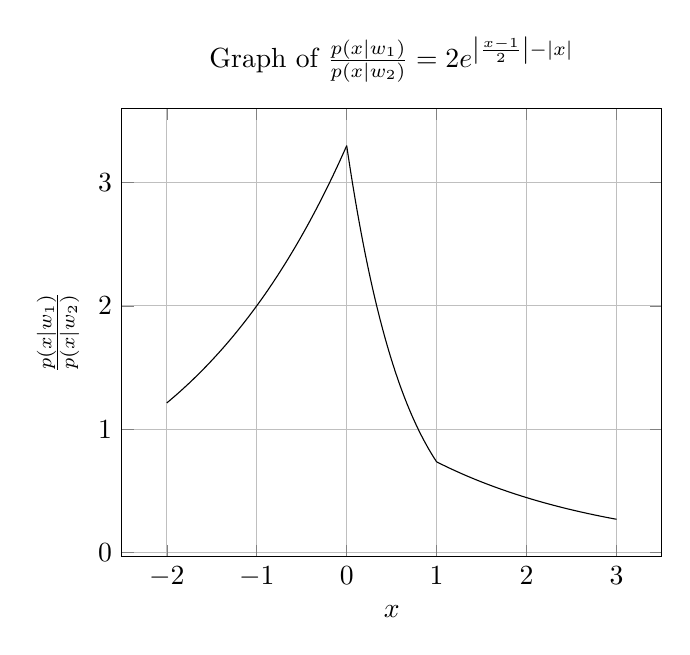
\begin{tikzpicture}
        \begin{axis}[
            domain=-2:3,
            samples=100,
            smooth,
            xlabel=\(x\),
            ylabel=\(\frac{p(x|w_1)}{p(x|w_2)}\),
            title={Graph of \( \frac{p(x|w_1)}{p(x|w_2)} = 2e^{\left| \frac{x - 1}{2} \right| - |x|} \)},
            grid=major
        ]
            % For x > 1
            \addplot[black, domain=1:3]{2*exp(-0.5*(x + 1))};
            
            % For 0 <= x <= 1
            \addplot[black, domain=0:1]{2*exp(-0.5*(3*x - 1))};
            
            % For x < 0
            \addplot[black, domain=-2:0]{2*exp(0.5*(1 + x))};
        \end{axis}
      \end{tikzpicture}
    \end{center}
\end{homeworkProblem}

\newpage

\begin{homeworkProblem}
  Consider the three-dimensional normal distribution $p(x|\omega) \sim N(\mu, \Sigma)$, where
  \[
    \mu = \begin{pmatrix}
      1 \\
      2 \\
      2 \\
    \end{pmatrix} \text{ and } \Sigma = \begin{pmatrix}
      1 & 0 & 0 \\
      0 & 5 & 2 \\
      0 & 2 & 5 \\
    \end{pmatrix}.
  \]

  \part{A}


  Find the probability density at the point $x_0 = (.5, 0, 1)^t$. \\

  \textbf{Solution}

  \[
    p(x_0|\omega) = 0.0082.
  \]

  \part{B}


  Construct the whitening transformation $A_{\omega}$. 
  Compute the matrices representing eigenvectors and eigenvalues, $\Phi$ and $\Lambda$.
  Next, convert the distribution to one centered on the origin with covariance matrix equal to the identity matrix, $p(x|\omega) \sim N(0, I)$.
  \\

  \textbf{Solution}

  We first normalize the mean by subtracting $x$ by $\mu$ and get $z = x - \mu$. We know $z \sim N(0, \Sigma)$.
  
  We then normalize the covariance matrix. We perform eigenvalue decomposition and get $\Sigma = \Phi\Lambda\Phi^T$, where
  \[
    \Phi \approx \begin{pmatrix}
      1 & 0 & 0 \\
      0 &  -0.7071 & 0.7071 \\
      0 &  0.7071 & 0.7071 \\
    \end{pmatrix} \text{ and } \Lambda = \begin{pmatrix}
      1 & 0 & 0 \\
      0 & 3 & 0 \\
      0 & 0 & 7 \\
    \end{pmatrix}.
  \]
  Let $A_w = \Phi\Lambda^{-\frac{1}{2}} \approx \begin{pmatrix}
    1.0000 & 0 & 0 \\
    0 & -0.4082 & 0.2673 \\
    0 & 0.4082 & 0.2673 \\
  \end{pmatrix}$. Then $A_w^T\Sigma A_w = \Lambda^{-\frac{1}{2}}\Phi^T\Phi\Lambda\Phi^T\Phi\Lambda^{-\frac{1}{2}} = I$.

  Thus, $y = A_w^Tz = A_w^T(x - \mu)$ is the normalization tranformation we are looking for. \\

  \part{C}


  Apply the same overall transformation to $x_0$ to yield a transformed point $x_w$. \\

  \textbf{Solution}
  \[
    x_w = A_w^T(x_0 - \mu) = (-0.5, 0.4082, -0.8018)^T.
  \]
  
  \pagebreak

  \part{D}


  By explicit calculation, confirm that the Mahalanobis distance from $x_0$ to the mean $\mu$
  in the original distributionis the same as for $x_w$ to $0$ in the transformed distribution. \\

  \textbf{Solution}

  \[
    r^2 = (x_0 - \mu)^T\Sigma^{-1}(x_0 - \mu) = 1.0595 = x_w^Tx_w.
  \]
  \\

  \part{E}

  Does the probability density remain unchanged under a general transformation?
  In other words, is $p(x_0|N(\mu, \Sigma)) = p(T^tx_0|N(T^t\mu, T^t\Sigma T))$ for some linear transform $T$?
  \\
  
  \textbf{Solution}

  Let $y = T^tx_0$. Notice that the Mahalanobis distance of the transformed distribution is
  \begin{align*}
    (T^tx_0 - T^t\mu)^t(T^t\Sigma T)^{-1}(T^tx_0 - T^t\mu)
    &= (x_0 - \mu)^tTT^{-1}\Sigma^{-1} (T^t)^{-1}T^t(x_0 - \mu) \\
    &= (x_0 - \mu)^t\Sigma^{-1} (x_0 - \mu),
  \end{align*}
  which remains the same. 
  However, since the transformation changed the covariance matrix from $\Sigma$ to $T^t\Sigma T$,
  the normalizing term of each distribution, $\frac{1}{|\Sigma|}$ and $\frac{1}{|T^t\Sigma T|}$, differs unless $|T| = \pm 1$.
  Since normalization is not perserved, the transformed probability density is not unchanged in general. \\


  \part{F}

  Prove that the whitening transform $A_w = \Phi\Lambda^{-1/2}$ when applied to a Gaussian distribution ensures that the final distribution has covariance proportional to the identity matrix $I$.
  Check whether normalization is perserved by the transformation.
  \\

  \textbf{Solution}

  Let there be a distribution $p(x|N(\mu, \Sigma))$, and let $y = A_w^tx$. 
  Then, 
  \begin{align*}
    \Sigma_y
    &= E[(y - \mu_y)(y - \mu_y)^t] \\
    &= E[(A_w^tx - A_w^t\mu)(A_w^tx - A_w^t\mu)^t] \\
    &= E[A_w^t(x - \mu)(x - \mu)^tA_w] \\
    &= A_w^t \Sigma A_w \\
    &= (\Lambda^{-1/2}\Phi^t)(\Phi\Lambda\Phi^t)(\Phi\Lambda^{-1/2}) \\
    &= I.
  \end{align*}
  Thus, we have shown that the covariance after the whitening transformation is indeed $I$.

  However, since 
  \[
    p(x|N(\mu, \Sigma)) = \frac{1}{\sqrt{(2\pi)^d |\Sigma|}}\exp\left(-\frac{1}{2}(x - \mu)^t\Sigma^{-1}(x - \mu)\right)
  \]
  but
  $p(y) = $
  \begin{align*}
    p(y) 
    &= \frac{1}{\sqrt{(2\pi)^d |\Sigma_y|}}\exp\left(-\frac{1}{2}(y - \mu_y)^t\Sigma_y^{-1}(y - \mu_y)\right) \\
    &= \frac{1}{\sqrt{(2\pi)^d}}\exp\left(-\frac{1}{2}(A_w^tx - A_w^t\mu)^t\Sigma_y^{-1}(A_w^tx - A_w^t\mu)\right) \\
    &= \frac{1}{\sqrt{(2\pi)^d}}\exp\left(-\frac{1}{2}(x - \mu)^tA_wA_w^t(x - \mu)\right) \\
    &= \frac{1}{\sqrt{(2\pi)^d}}\exp\left(-\frac{1}{2}(x - \mu)^t\Sigma^{-1}(x - \mu)\right),
  \end{align*}
  the distribution differs as the normalization fail to hold unless $|\Sigma| = \pm 1$.
\end{homeworkProblem}

\newpage

\begin{homeworkProblem}
    Let the components of the vector $x = (x_1, \dots, x_d)^t$ be binary valued and
  $P(\omega_j)$ be the prior probability for the state of nature $\omega_j$ and $j = 1, \dots, c$. Now define
  \[
    p_{ij} = Prob(x_i = 1|\omega_j) \quad i = 1, \dots , d \quad j = 1, \dots, c,
  \]
  with the components of $x_i$ being statistically independent for all $x$ in $\omega_j$.

  \begin{enumerate}
    \item[(a)] Interpret in words the meaning of $p_{ij}$.

    \textbf{Solution}

    $p_{ij}$ is the probability that $x_i$ is $1$ given the state of nature is $w_j$.
    
    \item[(b)] Show that the minimum probability of error is achieved by the following decision
    rule: Decide $\omega_k$ if $g_k(x) \geq g_j (x)$ for all $j$ and $k$, where
    \[
      g_j(x) = \sum^d_{i = 1} x^i \ln{\frac{p_{ij}}{1 - p_{ij}}} + \sum^d_{i = 1} \ln(1 - p_{ij}) + \ln{P(\omega_j)}.
    \]
    
    \textbf{Solution}

    Let $g^*(x)$ be the decision rule of minimum probability error. 
    We first note that

    \[
      P_{X_i|Y}(x_i|\omega_j) = \begin{cases}
        p_{ij} & x_i = 1 \\
        1 - p_{ij} & x_i = 0
      \end{cases} = p_{ij}^{x_i}(1 - p_{ij})^{1 - x_i}.
    \]
    Then,
    \begin{align*}
      g^*(x)
      &= \underset{\omega_j}{\arg\max} \, P_{Y|X}(\omega_j|x) \\
      &= \underset{\omega_j}{\arg\max} \, P_{X|Y}(x|\omega_j)P(\omega_j) \\
      &= \underset{\omega_j}{\arg\max} \, \ln P_{X|Y}(x|\omega_j) + \ln P(\omega_j) \\
      &= \underset{\omega_j}{\arg\max} \, \ln (\underset{i}\Pi{P_{X_i|Y}(x_i|\omega_j)}) + \ln P(\omega_j) \\
      &= \underset{\omega_j}{\arg\max} \, \ln (\underset{i}\Pi{p_{ij}^{x_i}(1 - p_{ij})^{1 - x_i}}) + \ln P(\omega_j) \\
      &= \underset{\omega_j}{\arg\max} \, \underset{i}\sum \ln ({p_{ij}^{x_i}(1 - p_{ij})^{1 - x_i}}) + \ln P(\omega_j) \\
      &= \underset{\omega_j}{\arg\max} \, \underset{i}\sum (x_i\ln (p_{ij}) + (1 - x_i)\ln (1 - p_{ij})) + \ln P(\omega_j) \\
      &= \underset{\omega_j}{\arg\max} \, \underset{i}\sum \left(x_i\ln \left(\frac{p_{ij}}{1 - p_{ij}}\right) + \ln (1 - p_{ij})\right) + \ln P(\omega_j) \\
      &= \underset{\omega_j}{\arg\max} \, \underset{i}\sum x_i\ln \left(\frac{p_{ij}}{1 - p_{ij}}\right) + \sum_i \ln (1 - p_{ij}) + \ln P(\omega_j).
    \end{align*}
  \end{enumerate}
\end{homeworkProblem}
\end{document}